\documentclass[../_main/handlingar.tex]{subfiles}

\begin{document}
\proposition{Inköp av ny spisfläkt till Edekvataköket}
Den nuvarande spisfläkten är i väldigt dåligt skick och bör därför bytas ut. Om fläkten förblir som den är idag kan vi få problem från huset p.g.a. matlukt i övriga huset. Styrelsen har kollat på olika förslag och anser att följande modell av fläkt är lämpad för köket i Edekvata.

\begin{center}
   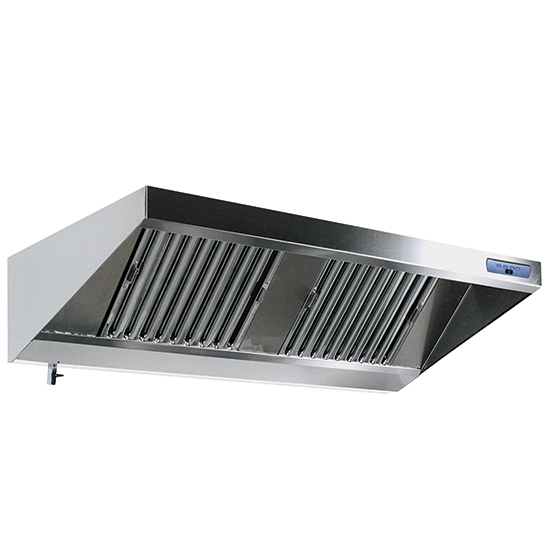
\includegraphics[width=8cm]{koksflakt.jpg}
\end{center}

Därför yrkar vi på
\begin{attsatser}
    \att köpa in en ny spisfäkt anpassad för storkök/resturang, liknande varianten ovan.
    \att bugeten för inköpet, frakt och installation sätts till 22000kr.
    \att kostnaden belastar utrustningsfonden.
    \att detta läggs på beslutsuppföljningen till HT/16 där sittande styrelsen står som ansvarig.
\end{attsatser}

\begin{signatures}{2}
    \ist
    \signature{Anders Nilsson}{Förvaltningschef}
    \signature{\ordf}{Ordförande}
\end{signatures}

\end{document}
